% ------------------------------------------------------------------------
% ------------------------------------------------------------------------
% Modelo UFSC para Trabalhos Academicos (tese de doutorado, dissertação de
% mestrado) utilizando a classe abntex2
%
% Autor: Alisson Lopes Furlani
% 	Modificações:
%	- 27/08/2019: Alisson L. Furlani, add pacote 'glossaries' para listas
% - 30/10/2019: Alisson L. Furlani, adjusted some spacing errors and changed math fonts
% - 17/01/2019: Alisson L. Furlani, updated certification page
% - 03/03/2020: Luiz F. P. Droubi, change file to be used as a template with R.
% ------------------------------------------------------------------------
% ------------------------------------------------------------------------

\documentclass[
	% -- opções da classe memoir --
	12pt,				% tamanho da fonte
	%openright,			% capítulos começam em pág ímpar (insere página vazia caso preciso)
	oneside,			% para impressão no anverso. Oposto a twoside
	a4paper,			% tamanho do papel.
	% -- opções da classe abntex2 --
	chapter=TITLE,		% títulos de capítulos convertidos em letras maiúsculas
	section=TITLE,		% títulos de seções convertidos em letras maiúsculas
	%subsection=TITLE,	% títulos de subseções convertidos em letras maiúsculas
	%subsubsection=TITLE,% títulos de subsubseções convertidos em letras maiúsculas
	% -- opções do pacote babel --
	english,			% idioma adicional para hifenização
	%french,				% idioma adicional para hifenização
	%spanish,			% idioma adicional para hifenização
	brazil				% o último idioma é o principal do documento
	]{abntex2}

\usepackage{setup/ufrnthesisA4-alf}

\addbibresource{bib/thesis.bib}
\addbibresource{bib/references.bib}
\addbibresource{bib/pkgs.bib}

\usepackage[table]{xcolor}
\let\newfloat\undefined
\usepackage{floatrow}
\floatsetup[table]{capposition=top}
\floatsetup[figure]{capposition=top}

\newcommand{\pkg}[1]{{\normalfont\fontseries{b}\selectfont #1}}
\let\proglang=\textsf
\let\code=\texttt


\newcommand{\bcenter}{\begin{center}}
\newcommand{\ecenter}{\end{center}}

\newcommand{\bapendices}{\begin{apendicesenv}}
\newcommand{\eapendices}{\end{apendicesenv}}

\newcommand{\banexos}{\begin{anexosenv}}
\newcommand{\eanexos}{\end{anexosenv}}

% ---
% Filtering and Mapping Bibliographies
% ---
\DeclareSourcemap{
	\maps[datatype=bibtex]{
		% remove fields that are always useless
		\map{
			\step[fieldset=abstract, null]
			\step[fieldset=pagetotal, null]
		}
		% remove URLs for types that are primarily printed
%		\map{
%			\pernottype{software}
%			\pernottype{online}
%			\pernottype{report}
%			\pernottype{techreport}
%			\pernottype{standard}
%			\pernottype{manual}
%			\pernottype{misc}
%			\step[fieldset=url, null]
%			\step[fieldset=urldate, null]
%		}
		\map{
			\pertype{inproceedings}
			% remove mostly redundant conference information
			\step[fieldset=venue, null]
			\step[fieldset=eventdate, null]
			\step[fieldset=eventtitle, null]
			% do not show ISBN for proceedings
			\step[fieldset=isbn, null]
			% Citavi bug
			\step[fieldset=volume, null]
		}
	}
}
% ---

% ---
% Informações de dados para CAPA e FOLHA DE ROSTO
% ---
% FIXME Substituir 'Nome completo do autor' pelo seu nome.
\autor{JOÃO VITOR FERREIRA CAVALCANTE}
% FIXME Substituir 'Título do trabalho' pelo título da trabalho.
\titulo{TÍTULO DE METAGENÔMICA}
% FIXME Substituir 'Subtítulo (se houver)' pelo subtítulo da trabalho.
% Caso não tenha substítulo, comente a linha a seguir.
  \subtitulo{SUBTÍTULO}
% FIXME Substituir 'XXXXXX' pelo nome do seu
% orientador.
\orientador{Rodrigo Juliani Siqueira Dalmolin}
% FIXME Se for orientado por uma mulher, comente a linha acima e descomente a linha a seguir.
% \orientador[Orientadora]{Nome da orientadora, Dra.}
% FIXME Substituir 'XXXXXX' pelo nome do seu
% coorientador. Caso não tenha coorientador, comente a linha a seguir.
% FIXME Se for coorientado por uma mulher, comente a linha acima e descomente a linha a seguir.
% \coorientador[Coorientadora]{XXXXXX, Dra.}
% FIXME Substituir '[ano]' pelo ano (ano) em que seu trabalho foi defendido.
\ano{2025}
% FIXME Substituir '[dia] de [mês] de [ano]' pela data em que ocorreu sua defesa.
\data{31 de Setembro de 2025}
% FIXME Substituir 'Local' pela cidade em que ocorreu sua defesa.
\local{NATAL - RN}
\instituicaosigla{UFRN}
\instituicao{Universidade Federal do Rio Grande do Norte}
% FIXME Substituir 'Dissertação/Tese' pelo tipo de trabalho (Tese, Dissertação).
\tipotrabalho{Defesa de Mestrado}
% FIXME Substituir '[mestre/doutor] em XXXXXX' pela grau adequado.
\formacao{Mestre em Bioinformática}
% FIXME Substituir '[mestrado/doutorado]' pelo nivel adequado.
\nivel{mestrado}
% FIXME Substituir 'Programa de Pós-Graduação em XXXXXX' pela curso adequado.
\programa{Programa de Pós-Graduação em Bioinformática}
% FIXME Substituir 'Campus XXXXXX ou Centro de XXXXXX' pelo campus ou centro adequado.
\centro{Instituto Metrópole Digital}
\preambulo
{%
\imprimirtipotrabalho~apresentada~ao~\imprimirprograma~da~\imprimirinstituicao.
}
% ---

% ---
% Configurações de aparência do PDF final
% ---
% alterando o aspecto da cor azul
\definecolor{blue}{RGB}{41,5,195}
% informações do PDF
\makeatletter
\hypersetup{
     	%pagebackref=true,
		pdftitle={\@title},
		pdfauthor={\@author},
    	pdfsubject={\imprimirpreambulo},
	    pdfcreator={LaTeX with abnTeX2},
		pdfkeywords={ufsc, latex, abntex2},
		colorlinks=true,       		% false: boxed links; true: colored links
    	linkcolor=black,%blue,          	% color of internal links
    	citecolor=black,%blue,        		% color of links to bibliography
    	filecolor=black,%magenta,      		% color of file links
		urlcolor=black,%blue,
		bookmarksdepth=4
}
\makeatother
% ---

% ---
% compila a lista de abreviaturas e siglas e a lista de símbolos
% ---

% Declaração das siglas
\siglalista{MS}{metagenômica \textit{shotgun}}
\siglalista{16S}{sequenciamento da subunidade ribossomal 16S de genomas bacterianos}
\siglalista{TDM}{transtorno depressivo maior}
\siglalista{DNA}{Ácido Desoxirribonucléico}
\siglalista{OTU}{unidades taxonômicas operacionais - do inglês \textit{operational taxonomic units}}
\siglalista{ASV}{variantes de sequência amplicon - do inglês \textit{amplicon sequence variant}}


% Declaração dos simbolos
\simbololista{C}{\ensuremath{C}}{Circunferência de um círculo}
\simbololista{pi}{\ensuremath{\pi}}{Número pi}
\simbololista{r}{\ensuremath{r}}{Raio de um círculo}
\simbololista{A}{\ensuremath{A}}{Área de um círculo}


% compila a lista de abreviaturas e siglas e a lista de símbolos
\makenoidxglossaries

% ---

% ---
% compila o indice
% ---
\makeindex
% ---

% ----
% Início do documento
% ----
\begin{document}

% Seleciona o idioma do documento (conforme pacotes do babel)
%\selectlanguage{english}
\selectlanguage{brazil}

% Retira espaço extra obsoleto entre as frases.
\frenchspacing

% Espaçamento 1.5 entre linhas
\OnehalfSpacing

% Corrige justificação
%\sloppy

% ----------------------------------------------------------
% ELEMENTOS PRÉ-TEXTUAIS
% ----------------------------------------------------------
% \pretextual %a macro \pretextual é acionado automaticamente no início de \begin{document}
% ---
% Capa, folha de rosto, ficha bibliografica, errata, folha de apróvação
% Dedicatória, agradecimentos, epígrafe, resumos, listas
% ---
% ---
% Capa
% ---
\imprimircapa
% ---

% ---
% Folha de rosto
% (o * indica que haverá a ficha bibliográfica)
% ---
\imprimirfolhaderosto*
% ---

% ---
% Inserir a ficha bibliografica
% ---
% http://ficha.bu.ufsc.br/
% \begin{fichacatalografica}
% 	\includepdf{Ficha_Catalografica.pdf}
% \end{fichacatalografica}
% ---

% ---
% Inserir folha de aprovação
% ---
\begin{folhadeaprovacao}
	\OnehalfSpacing
	% \centering
	\begin{center}
	\imprimirautor\\%
	\vspace*{10pt}
	\textbf{\imprimirtitulo}%
	\ifnotempty{\imprimirsubtitulo}{:~\imprimirsubtitulo}\\%
	%		\vspace*{31.5pt}%3\baselineskip
	\vspace*{\baselineskip}
	\end{center}
	%\begin{minipage}{\textwidth}
	\imprimirtipotrabalho~apresentada~ao~\imprimirprograma~da~\imprimirinstituicao\\
	%\end{minipage}%
	\bigskip\newline
	\textbf{Área de Concentração}:~Bioinformática\newline%
	\textbf{Linha de Pesquisa}:~Biologia de Sistemas\newline%
	\imprimirorientadorRotulo:~\imprimirorientador\newline%
	\begin{flushright}
	Natal, \imprimirdata.
	\end{flushright}
	\vspace*{\baselineskip}
  %   % Prof. Examinador 1, Dr.\\
  % Universidade Federal do Rio Grande do Norte - UFRN\\
  % \vspace*{\baselineskip}
  %   % Prof. Examinador 2, Dr.\\
  % Universidade Federal dos Externos - UFE\\
  % \vspace*{\baselineskip}
  % 
	\vspace*{2\baselineskip}
	% \begin{minipage}{\textwidth}
	% 	Certificamos que esta é a \textbf{versão original e final} do trabalho de conclusão que foi julgado adequado para obtenção do título de \imprimirformacao.\\
	% \end{minipage}
	%    \vspace{-0.7cm}
	\centering{\textbf{BANCA EXAMINADORA}}
	\assinatura{\OnehalfSpacing Prof. Dr. \imprimirorientador \\ \footnotesize{\imprimirinstituicao \\ (Presidente)}}
    \assinatura{Prof. Dr. Examinador 1 \\ \footnotesize{Universidade Federal do Rio Grande do Norte \\ (Examinador Interno do Programa)}}
    \assinatura{Prof. Dr. Examinador 2 \\ \footnotesize{Universidade Federal dos Externos \\ (Examinador Externo à Instituição)}}
  	%	\ifnotempty{\imprimircoorientador}{
	%	\assinatura{\imprimircoorientador \\ \imprimircoorientadorRotulo \\
	%		\imprimirinstituicao~--~\imprimirinstituicaosigla}
	%	}
	% \newpage
	\vspace*{\fill}
	\centering
\end{folhadeaprovacao}
% ---

% ---
% Dedicatória
% ---
% \begin{dedicatoria}
% 	\vspace*{\fill}
% 	\noindent
% 	\begin{adjustwidth*}{}{5.5cm}
% 		\raggedleft
% 		Este trabalho é dedicado a algumas pessoas.
% 	\end{adjustwidth*}
% \end{dedicatoria}
% ---

% ---
% Agradecimentos
% ---
\begin{agradecimentos}
	Gostaria de agradecer sinceramente a todos os que colaboraram à execução\\
deste trabalho.
\end{agradecimentos}
% ---

% ---
% Epígrafe
% ---
\begin{epigrafe}
	\vspace*{\fill}
	\begin{flushright}
		\textit{``Eppur si muove!''\\
(Galileu Galilei, 1633)}
	\end{flushright}
\end{epigrafe}
% ---

% ---
% RESUMOS
% ---

% resumo em português
\setlength{\absparsep}{18pt} % ajusta o espaçamento dos parágrafos do resumo
\begin{resumo}
	\SingleSpacing
  No resumo são ressaltados o objetivo da pesquisa, o método utilizado, as discussões e os resultados com destaque apenas para os pontos principais. O resumo deve ser significativo, composto de uma sequência de frases concisas, afirmativas, e não de uma enumeração de tópicos. Não deve conter citações. Deve usar o verbo na voz ativa e na terceira pessoa do singular. O texto do resumo deve ser digitado, em um único bloco, sem espaço de parágrafo. O espaçamento entre linhas é simples e o tamanho da fonte é 12. Abaixo do resumo, informar as palavras-chave (palavras ou expressões significativas retiradas do texto) ou, termos retirados de thesaurus da área. Deve conter de 150 a 500 palavras. O resumo é elaborado de acordo com a NBR 6028.

  \textbf{Palavras-chave}:
    Palavra-chave 1.
    Palavra-chave 2.
  \end{resumo}
% resumo em inglês
\begin{resumo}[Abstract]
	\SingleSpacing
	\begin{otherlanguage*}{english}
		Resumo traduzido para outros idiomas, neste caso, inglês. Segue o formato do resumo feito na língua vernácula. As palavras-chave traduzidas, versão em língua estrangeira, são colocadas abaixo do texto precedidas pela expressão ``Keywords'', separadas por ponto.

		\textbf{Keywords}:
	      Keyword 1.
        Keyword 2.
    	\end{otherlanguage*}
\end{resumo}
%% resumo em francês
%\begin{resumo}[Résumé]
% \begin{otherlanguage*}{french}
%    Il s'agit d'un résumé en français.
%
%   \textbf{Mots-clés}: latex. abntex. publication de textes.
% \end{otherlanguage*}
%\end{resumo}
%
%% resumo em espanhol
%\begin{resumo}[Resumen]
% \begin{otherlanguage*}{spanish}
%   Este es el resumen en español.
%
%   \textbf{Palabras clave}: latex. abntex. publicación de textos.
% \end{otherlanguage*}
%\end{resumo}
%% ---

{%hidelinks
	\hypersetup{hidelinks}
	% ---
	% inserir lista de ilustrações
	% ---
	\pdfbookmark[0]{\listfigurename}{lof}
	\listoffigures*
	\cleardoublepage
	% ---

	% ---
	% inserir lista de quadros
	% ---
	% \pdfbookmark[0]{\listofquadrosname}{loq}
	% \listofquadros*
	% \cleardoublepage
	% ---

	% ---
	% inserir lista de tabelas
	% ---
	\pdfbookmark[0]{\listtablename}{lot}
	\listoftables*
	\cleardoublepage
	% ---

	% ---
	% inserir lista de abreviaturas e siglas (devem ser declarados no preambulo)
	% ---
	\imprimirlistadesiglas
	% ---

	% ---
	% inserir lista de símbolos (devem ser declarados no preambulo)
	% ---
	% \imprimirlistadesimbolos
	% ---

	% ---
	% inserir o sumario
	% ---
	\pdfbookmark[0]{\contentsname}{toc}
	\tableofcontents*
	\cleardoublepage

}%hidelinks
% ---

% ---

% ----------------------------------------------------------
% ELEMENTOS TEXTUAIS
% ----------------------------------------------------------
\textual

\chapter{Introdução}\label{intro}

\section{Visão Geral - Metagenômica}\label{visuxe3o-geral---metagenuxf4mica}

A história da vida microscópica, ou microbiana, no planeta Terra supera a história da vida macroscópica por milhares de anos (\textbf{ref}). A metagenômica surge como uma abordagem que possibilita descobertas acerca da vida microbiana através do sequenciamento genético. Avanços no que viria eventualmente a se tornar a metagenômica surgem ainda nos anos 90, com o primeiro sequenciamento de genoma completo de um organismo de vida livre, a bactéria \emph{Haemophilus influenza} \autocite{wooley2010}. Esse ponto na história científica marca o primeiro uso bem sucedido do que vem a ser chamado de \emph{whole-genome shotgun}, ou sequenciamento de genoma completo, no qual a amostra possui seu conteúdo genético fragmentado em \emph{reads}, ou leituras, que são então sequenciadas. Essa técnica viria a ser refinada e aplicada para amostras ambientais, seja este ambiente uma amostra de solo florestal ou uma biópsia intestinal. Nessa nova técnica se buscou sequenciar o conteúdo genético que compreenda os diferentes microorganismos presentes em tais amostras, originando assim o que será aqui descrito como \gls{MS}.

No entanto, o estudo de comunidades microbianas se populariza de fato com uma técnica que não busca capturar o conteúdo genético total de uma amostra, mas apenas uma subregião de seu \gls{DNA} ribossomal que possua ao mesmo tempo regiões conservadas, capaz de serem passíveis de anelamento por \emph{primers}, e regiões hipervariáveis, capazes de distinguir um microorganismo de outro. Em bactérias o ribotipo selecionado foi o \gls{DNA} que codifica a subunidade 16S, que é amplificada e então sequenciada. O \gls{16S}, também denominado metataxonômica \autocite{marchesi2015}, possibilitou uma maneira simples, e pouco computacionalmente intensiva quando comparada à \gls{MS} (\textbf{ref}), para realizar identificação de táxons bacterianos em uma amostra ambiental. Ademais, técnicas computacionais posteriores ultimamente facilitariam a conexão de informação funcional às abundâncias taxonômicas obtidas através desta técnica.

Dessa maneira, possuímos atualmente, duas possíveis abordagens para se estudar comunidades microbianas, a \gls{MS} e o \gls{16S}. Essas abordagens, por se basearem de aspectos distintos do microbioma, tipicamente são utilizadas de forma separada - e não integrativa - por estudos. Apesar disso, a integração de dados provenientes das duas abordagens pode auxiliar a remover vieses experimentais específicos de cada técnica, e, dessa maneira, conferir maior confiabilidade aos resultados \autocite{yue2023}.

\section{O Ecossistema computacional em Metagenômica}\label{o-ecossistema-computacional-em-metagenuxf4mica}

\section{Visão Geral - Transtorno Depressivo Maior}\label{visuxe3o-geral---transtorno-depressivo-maior}

\section{O Eixo Microbiota-Cérebro e o TDM}\label{o-eixo-microbiota-cuxe9rebro-e-o-tdm}

\chapter{Objetivos}\label{obj}

\section{Geral}\label{geral}

Obter uma visão geral do ecossistema computacional em metagenômica atual e como ele se associa
com princípios de desenvolvimento de software científico, desenvolvendo então uma metodologia
para dados de \{MS\} que possibilite uma análisa metagenômica compreensiva.
Por fim, se baseando em parte nessa nova metodologia, analisar dados da microbiota intestinal de pacientes com \gls{TDM} e trazer novas descobertas acerca da relação da enfermidade com aspectos metabólicos da microbiota.

\section{Específicos}\label{especuxedficos}
\begin{itemize}
\tightlist
\item
  Avaliar o atual ferramentário computacional para dados de metagenômica e sua adesão a princípios de desenvolvimento de software sustentável.
\item
  Desenvolver uma metodologia robusta, flexível e acessível para análise de dados de \gls{MS}.
\item
  Realizar uma meta-análise da microbiota intestinal de pacientes com \gls{TDM}, focando em aspectos metabólicos e funcionais.
\end{itemize}
\chapter*{CAPÍTULO 1}\label{cap1}
\addcontentsline{toc}{chapter}{CAPÍTULO 1}
\begin{center}
\textbf{Artigo: Bridging the Gaps in Meta-Omic Analysis: Workflows and Reproducibility}
\bigskip\newline
Escrito por: João Vitor Ferreira Cavalcante, Iara Dantas de Souza, Diego Arthur de Azevedo Morais e Rodrigo Juliani Siqueira Dalmolin
\bigskip\newline
\textit{Artigo publicado no periódico OMICS: A Journal of Integrative Biology}

\end{center}
\begin{fichacatalografica}
    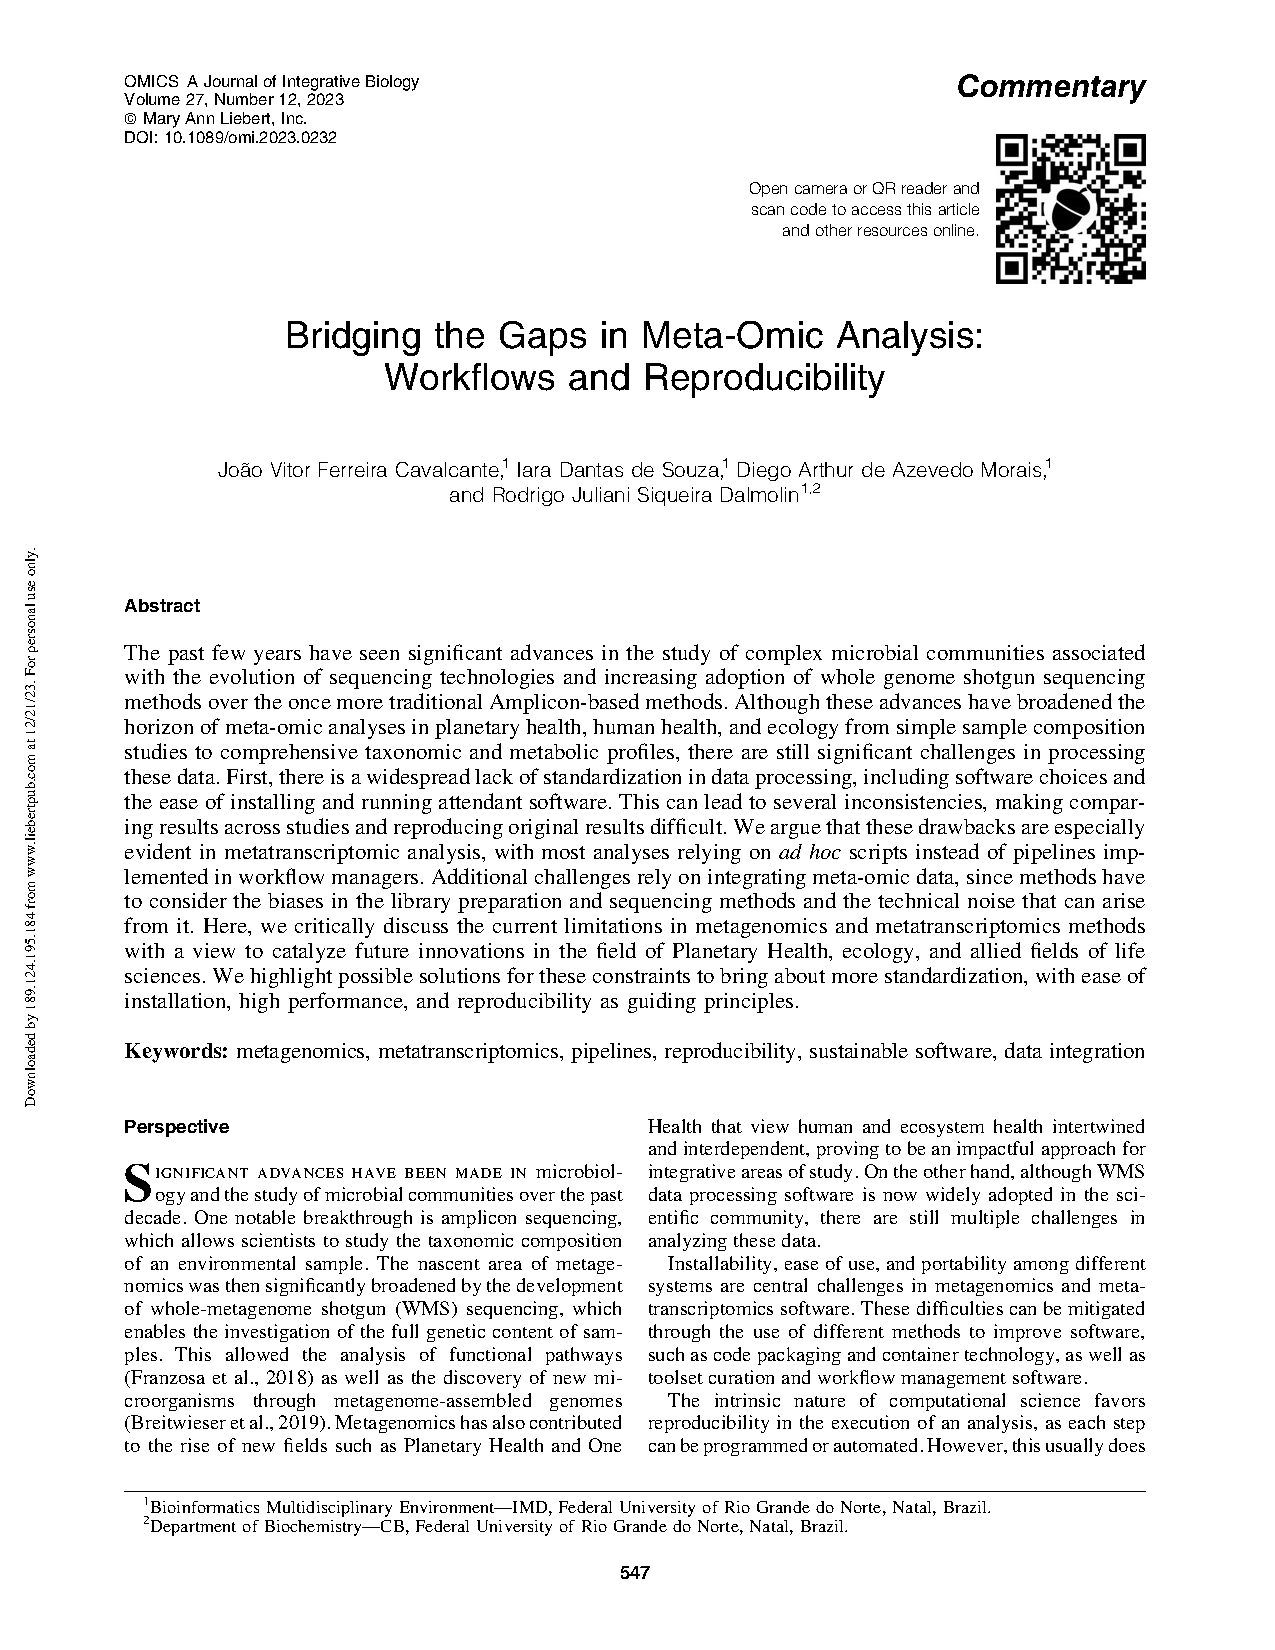
\includepdf[pages={1-}]{papers/paper1.pdf}
\end{fichacatalografica}
\chapter*{CAPÍTULO 2}\label{cap2}
\addcontentsline{toc}{chapter}{CAPÍTULO 2}
\begin{center}
\textbf{Artigo: EURYALE: A versatile Nextflow pipeline for taxonomic classification and functional annotation of metagenomics data}
\bigskip\newline
Escrito por: João Vitor Ferreira Cavalcante, Iara Dantas de Souza, Diego Arthur de Azevedo Morais e Rodrigo Juliani Siqueira Dalmolin
\bigskip\newline
\textit{Artigo a ser submetido no periódico BioSystems}

\end{center}
\begin{fichacatalografica}
    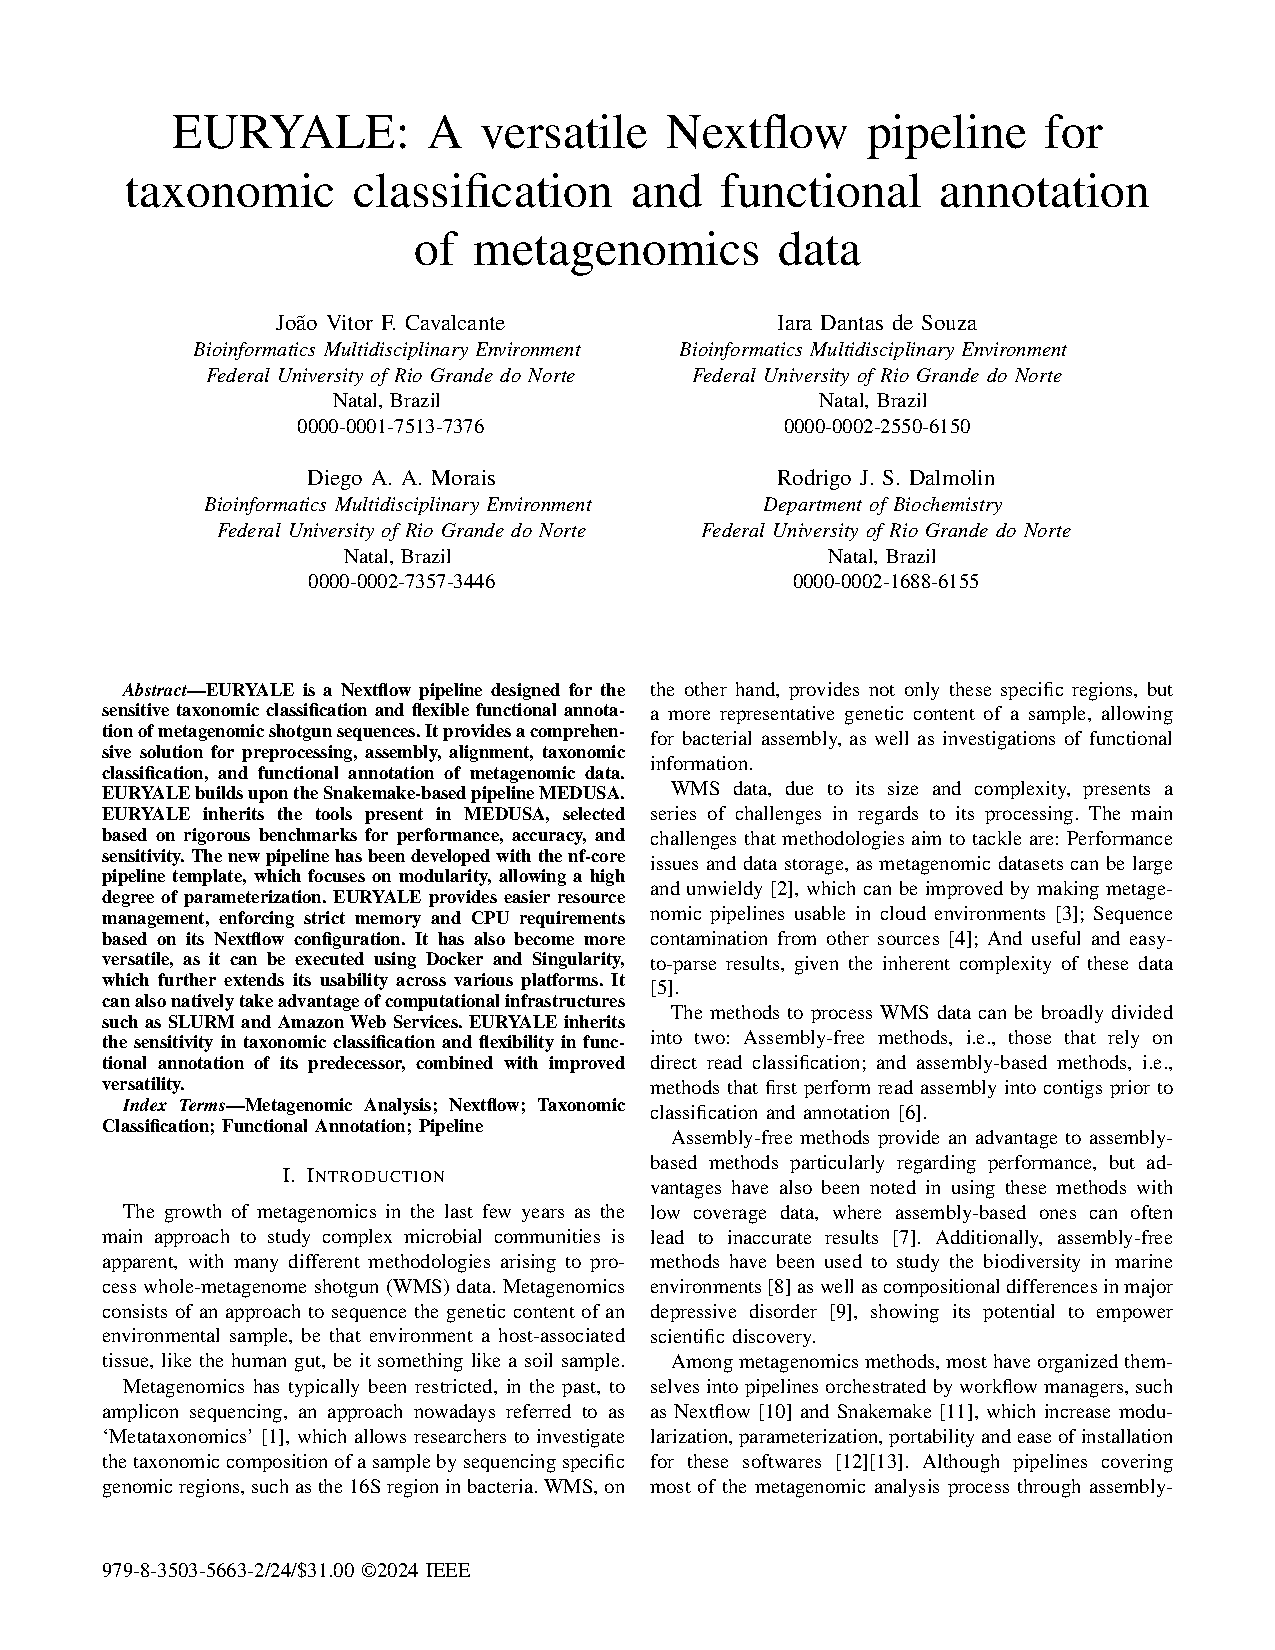
\includepdf[pages={1-}]{papers/paper2.pdf}
\end{fichacatalografica}
\chapter*{CAPÍTULO 3}\label{cap3}
\addcontentsline{toc}{chapter}{CAPÍTULO 3}
\begin{center}
\textbf{Artigo: Metagenomic meta-analysis reveals altered metabolic profiles in Major Depressive Disorder patients}
\bigskip\newline
Escrito por: João Vitor Ferreira Cavalcante, Julia Apolonio Amorim, Vasiliki Lagou e Rodrigo Juliani Siqueira Dalmolin
\bigskip\newline
\textit{Artigo a ser submetido no periódico Journal of Affective Disorders}

\end{center}
\chapter{Discussão}\label{disc}

blablabla

\chapter{Conclusão}\label{conclusuxe3o}

As conclusões devem responder às questões da pesquisa, em relação aos objetivos
e às hipóteses. Devem ser breves, podendo apresentar recomendações e sugestões
para trabalhos futuros.

\postextual

\begingroup

\printbibliography[title=REFERÊNCIAS]

\endgroup

\markboth{Referências}{REFERÊNCIAS}

% ----------------------------------------------------------
% Glossário
% ----------------------------------------------------------
%
% Consulte o manual da classe abntex2 para orientações sobre o glossário.
%
%\glossary

%---------------------------------------------------------------------
% INDICE REMISSIVO
%---------------------------------------------------------------------
%\phantompart
%\printindex
%---------------------------------------------------------------------

\end{document}
